% !TeX root = ../../thesis.tex
\chapter{Phase field method} \label{ch_introPF}

\section{General introduction}
Phase field method is a diffuse-interface approach to solving moving-boundary problems. In materials science it is usually used as meso-scale method. It has numerous applications such as e.g. (multi-component) solidification, grain growth, Ostwald ripening, solid-solid phase transitions (martensitic, precipitation, spinodal...), two-phase flow, nucleation, wetting and much more. 

The method is based on the principle of total system energy minimization. The free energy density of the system is a function of all the possibly mutually coupled physical fields, including the fields representing the phases. These are typically called phase fields, order parameters or continuum fields. The other (bulk) physical fields can be e.g. concentration, temperature, electric charge or others. The total energy of the system is then spatial integral of the free energy density over the simulation domain - the free energy functional.

The governing equation(s) for the phase fields are derived using principles of variational calculus, which ensure the fields evolution so that the free energy functional is minimized along the direction of steepest descent, i.e. the most likely way towards the equilibrium. Additionally, the curvature driving force and the possible coupling with the bulk fields are represented. That is the reason for high versatility of the method and its capability to simulate coupled multiphysics. 

Due to the thermodynamic nature of the method, the interface energy is naturally included as an input parameter. Multigrain or multiphase systems with interfaces of various properties can be simulated with multi phase field models. Some of these allow to include also inclination dependence of interface energy. In fact, it was phase field simulation which revealed the paramount importance of interface energy anisotropy in pattern formation during dendritic solidification~\cite{Kobayashi1993}.

A phase (or phases) in an inhomogeneous system is described by a continuous function (called phase field, order parameter or continuum field), having different constant values in the bulk of the phases (typically 1 and 0 or 1 and -1). At the interface between phases, the phase field varies smoothly between the values and the interface region is thus characterized by a certain width, as sketched in Figure~\ref{fig_PFintro_diffuse_interface}. This interface width is an important input parameter in phase field models. In quantitative phase field models, the model behavior is in principle not affected by the particular value of interface width chosen, which allows to make quantitative simulations at mesoscale (whereas the real interface width is in the order of units of nm).

\begin{figure}
	\centering
	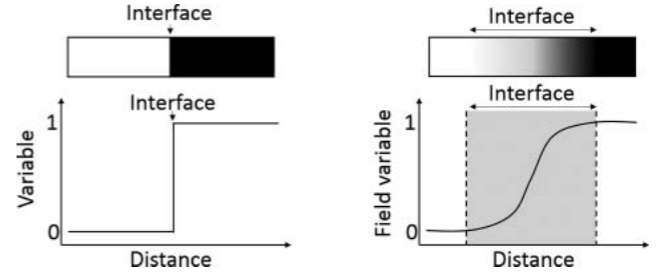
\includegraphics[width = 0.6\textwidth]{chapters/03PFintro/image/diffuse_interface_Bellemans2017}
	\caption[Interface width in phase field method]{Illustration of the diffuse interface in phase field method (on the right) and the comparison to an actual, sharp interface (on the left).~\cite{Bellemans2017}}
	\label{fig_PFintro_diffuse_interface}
\end{figure}

The governing equations for the phase fields are typically either conservative (Cahn-Hilliard type of equation, conserving volume) or non-conservative (Allen-Cahn type of equation). The latter is more relevant for this work. In the following, no coupling to other physical fields is assumed.

\section{Allen-Cahn equation for two-phase system}
It was shown that the Allen-Cahn equation is a diffuse-interface approximation of a curvature-driven system (even for anisotropic interface energy~\cite{Elliott1996}). It represents evolution of a non-conserved field $\eta(\mathbf{r})$ in a domain $\Omega\in\mathbb{R}^3$ with boundary $\partial\Omega$ and can be written as
\begin{align}
	\frac{\partial \eta}{\partial t} = -L\frac{\delta F}{\delta \eta} \quad &\mathrm{in \,\Omega}\\
	\nabla\eta\cdot\bm{n} = 0 \quad &\mathrm{at \, \partial\Omega}\,,
\end{align}
where $L$ is a positive constant and the function $\frac{\delta F}{\delta \eta}$ stands for functional derivative of the free energy functional $F$. The functional is an integral with free energy density $f(\eta,\nabla\eta)=f_{hom}(\eta)+f_{int}(\nabla\eta)$ comprising of the homogeneous and interfacial free energy densities
\begin{align}
	F 	&= \int_V f_{hom}(\eta)+f_{int}(\nabla\eta) \mathrm{d}V\\
		&= \int_V m \eta^2(1-\eta)^2 + \frac{\kappa}{2}|\nabla\eta|^2 \mathrm{d}V
\end{align}
with positive constants $m,\kappa$ being the double barrier height and gradient energy coefficient, respectively. The homogeneous free energy density $f_{hom}$ in the form of the double-well function assures two stable states for the field variable in values 0 and 1. The gradient energy contribution is lessened by the diffuse interface widening, whereas conversely the homogeneous free contribution is lessened by its narrowing. When minimizing the full integral, a balance between the two effects is reached in equilibrium.

As described in more detail in the Appendix~\ref{ch_appendix_functional_derivative}, the functional derivative is computed as
\begin{equation}
	\frac{\delta F}{\delta \eta} = \left[ \frac{\partial f}{\partial \eta_p} - \nabla\cdot\frac{\partial f}{\partial(\nabla \eta_p)} \right] \,
\end{equation}
where $\nabla\cdot\partial f/\partial(\nabla \eta_p)$ is divergence of vector field $\partial f/\partial(\nabla \eta_p)$ defined by relation
\begin{equation}
	\frac{\partial f}{\partial(\nabla \eta_p)} = \frac{\partial f}{\partial(\partial_x\eta_p)}\mathbf{n}_x + \frac{\partial f}{\partial(\partial_y \eta_p)}\mathbf{n}_y + \frac{\partial f}{\partial(\partial_z \eta_p)}\mathbf{n}_z
\end{equation}
with $\partial_x,\partial_y,\partial_z$ being operators for unidirectional derivatives in the corresponding directions and $\mathbf{n}_x,\mathbf{n}_y,\mathbf{n}_z$ coordinate base vectors. 

When applied applied to the above functional, it will result in the Allen-Cahn equation 
\begin{align}
	\frac{\partial \eta}{\partial t} &= -L[f_{hom}'(\eta) - \kappa\nabla^2\eta]\\
	 &=-L[2m\eta(1-\eta)(1-2\eta) - \kappa\nabla^2\eta] \,.
\end{align}

In equilibrium, the interface is static, $\partial \eta/\partial t = 0$, which means that the forces narrowing and widening the interface are in balance, i.e. $f_{hom}'(\eta) = \kappa\nabla^2\eta$, or equivalently (in 1D)
\begin{equation}
	2\eta(1-\eta)(1-2\eta) = \frac{\kappa}{m}\frac{\partial^2 \eta}{\partial x^2} \,.
\end{equation}
Solution to this equation provides the equilibrium profile of the phase field (centered in $x=0$), which in this case is the following sigmoid function
\begin{equation}
	\eta(x)=\frac{1}{2}\mathrm{tanh}\left(\sqrt{\frac{m}{2\kappa}}x\right) \,.
\end{equation}

The equilibrium also implies, that the homogeneous and interfacial energies are equal except for a constant, i.e. $f_{hom}=f_{int} + C$, which can be shown to be zero $C=0$ (see e.g.~\cite{Moelans2008}).

Interface width $l_{int}$ (unit \unit{\m}) can be defined using the reciprocal maximal slope in the interface (present in $\eta=0.5$)
\begin{equation}\label{eq_def_IW_fund_formula}
	l_{int} = \frac{1}{\mathrm{d}\eta/\mathrm{d}x|_{max}}=\left.\frac{1}{\sqrt{2 f_{hom}/\kappa}}\right|_{\eta=0.5} = 2\sqrt{2}\sqrt{\frac{\kappa}{m}} \,,
\end{equation}
where the relation $\mathrm{d}\eta/\mathrm{d}x=\sqrt{2 f_{hom}/\kappa}$ is derived from $f_{hom}=f_{int}$.

The excess free energy $\sigma$ (the \textit{interface energy}, unit \unit{\J/\m^2}) at a flat interface can be computed as an 1D integral of the free energy density  along perpendicular line through the interface
\begin{equation} \label{eq_def_IE_fundamental}
	\sigma = \int_{-\infty}^{+\infty} f_{hom} + \frac{\kappa}{2}|\nabla\eta|^2 \mathrm{d}x \,.
\end{equation}
From $f_{hom}=f_{int}$ it can be written $\mathrm{d}x = \sqrt{\kappa/2 f_{hom}}\mathrm{d}\eta$, which allows to solve~\eqref{eq_def_IE_fundamental} by substitution as follows
\begin{align} 
	\sigma =& \int_{-\infty}^{+\infty} 2f_{hom} \mathrm{d}x \\
			=& \int_{0}^{1} \sqrt{2 f_{hom}\kappa} \mathrm{d}\eta \\ 
\label{eq_def_IE_fund_formula}			
			=& \frac{\sqrt{2}}{6}\sqrt{m\kappa}  \,. 
\end{align}

In practice, the model is parameterized by the interface width $l_{int}$ and interface energy $\sigma$, from which the model parameters $m,\kappa $ must be computed. The necessary formulas are obtained from \eqref{eq_def_IW_fund_formula} and \eqref{eq_def_IE_fund_formula} as
\begin{align}
\label{eq_def_kappa_fund_formula} 	\kappa 	&= \frac{3}{2}\sigma l_{int} \\
			m 		&= 12\frac{\sigma}{l_{int}}
\end{align}

The $l_{int}$ is chosen depending on the scale of the problem, disregarding the real physical interface width. 

As shown in~\cite{Moelans2008}, the following equality between the model parameters and the interface mobility $\mu$ holds
\begin{equation}
	\mu\sigma = L\kappa \,,
\end{equation}
which allows to express the phase field kinetic coefficient as
\begin{equation}\label{eq_def_L_fund_formula}
	L = \frac{2}{3}\frac{\mu}{l_{int}}\,,
\end{equation}
where the equation~\eqref{eq_def_kappa_fund_formula} was used.


\section{Allen-Cahn equation for two-phase system including anisotropic interface energy}
	\subsection{Fundamentals}
	The most straightforward way to introduce anisotropy in the interface energy in the model is to make either of the model parameters $\kappa, m$ a function of the inclination angle respecting both the anisotropy function and the defining parameter relations. 
	
	Tschukin \cite{Tschukin2017} proposes the terminology of \textit{classical} and \textit{natural} models (corresponding to the notation VIW and VIE, respectively, as used by Fleck~\cite{Fleck2011}, standing for \textit{Variable Interface Width} and \textit{Variable Interface Energy}). The classical models~\cite{Kobayashi1993,McFadden1993,Taylor1998,Eggleston2001,Wheeler2006}, introduce anisotropy in the gradient energy coefficient $\kappa$, whereas the natural models~\cite{Ma2006,Torabi2009,Fleck2011,Moelans2008} in both the gradient energy coefficient $\kappa$ and homogeneous energy density barrier $m$. The main difference between the classical and natural formulations is that in the first case the diffuse interface width varies proportionally to the local interface energy (see equation~\eqref{eq_def_IW_fund_formula}), whereas in the latter the interface width can be decoupled from the interface energy and the interface width maintained constant (see~\eqref{eq_def_IW_fund_formula} and \eqref{eq_def_IE_fund_formula}). Below, more details are provided on both model formulations.
	
	Let's assume that the interface energy is inclination-dependent in the following form (in 2D)
	\begin{equation}\label{eq_def_IEaniso_PFintro}
		\sigma(\theta)=\sigma_0 h(\theta) \,,
	\end{equation}
	with the inclination angle $\theta$ of the interface normal $\bm{n}=[n_x,n_y]^\mathrm{T}$ being defined as $\theta = \mathrm{atan2d}(n_y/n_x)$ and $\sigma_0$ constant with physical dimensions \unit{\J/\m^2}. The interface normal is defined from phase field as
	\begin{equation}
		\bm{n} = \frac{\nabla\eta}{|\nabla\eta|} \,.
	\end{equation}
	
	First, a classical model with anisotropy only in $\kappa $ will be developed. The equations~\eqref{eq_def_IE_fund_formula} and~\eqref{eq_def_IEaniso_PFintro} are combined 
	\begin{equation}
		\sigma(\theta) = \sigma_0 h(\theta) = \frac{\sqrt{2}}{6}\sqrt{m\kappa(\theta)}
	\end{equation}
	and allow to express the anisotropic $\kappa(\theta)$
	\begin{equation}
		\kappa(\theta) = \kappa_0 [h(\theta)]^2 \quad \mathrm{and} \quad \sigma_0=(\sqrt{2}/6)\sqrt{m\kappa_0} \,,
	\end{equation}
	which recovers the interface energy anisotropy~\eqref{eq_def_IEaniso_PFintro}.
	
	Recall that $\theta=\theta(\bm{n}(\nabla\eta))$, hence the $\theta$ dependence in (any) model parameter implies that in the governing equations new terms arise from the divergence part of the functional derivative $\nabla\cdot\partial f/\partial(\nabla \eta_p)$, where the free energy density is taken derivative of with respect to the gradient components.
	
	This anisotropy implementation implies that the interface width $l_{int}$ varies proportionally to the interface energy (see~\eqref{eq_def_IW_fund_formula}), which must be taken into account in practice so that there are no excessively large or narrow interfaces in the domain. Additionally, the interface width variation introduces nonphysical anisotropy in the kinetic coefficient $L$ (see~\eqref{eq_def_L_fund_formula}), which should be compensated in the formula for $L$.
	
	In strongly anisotropic systems, the variable interface width poses a practical problem. However, it can be prevented by including the anisotropy also in the parameter $m$. When the anisotropy is assigned in the natural model formulation as
	\begin{align}
		\kappa(\theta) 	&= \kappa_0 h(\theta) \\
		m(\theta) 		&= m_0 h(\theta) \,,
	\end{align}
	the interface width is constant $l_{int}=2\sqrt{2}\sqrt{\frac{\kappa_0}{m_0}} $ (see~\eqref{eq_def_IW_fund_formula}) and the following relation holds as well
	\begin{equation}
		\sigma_0 h(\theta) = \frac{\sqrt{2}}{6}\sqrt{m(\theta)\kappa(\theta)} \,.
	\end{equation}
	Because both $\kappa,m$ depend on $\theta$, even more terms derive from the divergence in the functional derivative, as described earlier. 

	Another notable approach uses Finsler geometry to replace the Euclidean metric in the simulation domain by an anisotropic one~\cite{Bellettini1996,Benes2003}. Formally, the anisotropic Allen-Cahn equation is then not much more complicated then the isotropic one, even though new terms arise as well. The interface width is constant, though.
	
	\subsection{Challenges and limitations}
	The main challenges come from the type of anisotropy function and from the strength of anisotropy. So far, it was implicitly assumed that the anisotropy function is continuous and twice-differentiable homogeneous function of order 1. In chapter~\ref{ch_anisoIEintro} the problem arising from forbidden angles was worked in some detail, but here it will be put into a context specific for phase field method.
	
	Generally, two types of singularities may occur on the Wulff shapes of the first order (for the terminology see section~\ref{sec_isol_aniso_particle}): corners and facets. These two depend on the following properties of the particular anisotropy function
	\begin{enumerate}
		\item (non-)convexity of the Frank's plot, i.e. $1/h(\theta)$ and
		\item (non-)differentiability with respect to the polar angle (typically presence of a cusp).
	\end{enumerate}
	The first produces corners (when non-convex) and the second facets (when non-differentiable). 
	
	The easiest solution to the non-differentiability is to replace the anisotropy function by such one, in which the cusps are a smooth tips. These functions are typically formulated in such a way, that the sharpness of the tip is scalable, but formally the function is always smooth. This allows to approximate the former anisotropy close enough while assuring validity of the formulas relying on the differentiability. This was employed for example in~\cite{Debierre2003,Loginova2004,Miura2013}.
	
	The non-convexity of the Frank's plot does not have so easy solution. It causes the governing equations to be ill-posed, which means that the solution to is either not existing, unique or does not depend continuously on the initial/boundary conditions. In this case the uniqueness is the problem, because it is not clear, whether a certain segment on the surface should align with the "ear" orientation or some on the Wulff plot of the first order. In practice, it causes corrugations of the phase field contour near the corners, see e.g.~\cite{Tschukin2017}. The ill-posedness can be removed by regularization (and thus the match in corners improved), the following approaches are known to the author
	\begin{enumerate}
		\item regularization of the anisotropy function~\cite{Taylor1998,Eggleston2001,Kobayashi2001},
		\item inclusion of higher order terms in expansion of interface energy in the free energy functional~\cite{Wheeler2006, Torabi2009, Tschukin2017},
		\item models incorporating the Finsler geometry do not need regularization~\cite{Bellettini1996,Benes2003},
		\item one study reports numerical regularization which occurred after using spectral solver~\cite{Toth2015}.
	\end{enumerate}
	All of the above approaches were successful in delivering cornered or faceted Wulff shapes of the first order and anisotropic crystals grown in either temperature or concentration field. These were the main applications of these models so far. Very likely, each of these will have its own limitations in the future applications, but currently the author is unaware of any systematic comparison of these in the literature and himself only implemented the approach 1. from the list, i.e. the regularization of anisotropy function.

\section{Allen-Cahn equations for multi-phase systems}
	\subsection{Historical context}
	Multi-phase field models emerged from the need to simulate systems with more than two phases. At first, these models were developed to simulate ideal grain growth in systems with isotropic grain boundary energy. That is a natural choice, because the grain coarsening is curvature driven and the Allen-Cahn equation approximates the mean curvature flow. The main characteristic of the multi-phase field models is that every grain or phase is characterized by it own field variable, which implies that these systems may contain many governing equations, even tens of thousands in large scale grain growth simulations~\cite{Yadav2018}.
	
	Even though there were published many model formulations, all those known to the author can be attributed to one of two main branches of development: one initiated by the work of Long-Qing Chen in 1994~\cite{Chen1994} and the other by Steinbach in 1996~\cite{Steinbach1996}. The most fundamental difference is that in Steinbach's branch, the field variables are interpreted as local phase fractions, whereas in the Chen's there is no direct physical interpretation of the field variables. For this reason, it is not accurate to call the latter multi-phase-field models (MPF), but the difference is rather technical and not obvious to broader scientific community. When there is the need to differentiate the two groups of models, the multi-continuum-field (CF) or multi-order-parameter model are the options to call the models in Chen's legacy.
	
	Both multi-phase-field and multi-continuum-field models were extensively developed beyond the ideal grain growth, and nowadays the two model families are comparable in terms of maturity and applicability. The models offer anisotropy in interface energy and kinetic coefficient (pair-wise isotropic as well as the inclination dependence), coupling to multi-component systems using the Onsager's theory, possibly employing the thermodynamic databases to express the concentration dependence of the free energy density. 
	
	Real interfaces (including the grain boundaries) exhibit anisotropic (inclination-dependent) interface energies ~\cite{Olmsted2009,Bulatov2014}, hence a significant effort was made to introduce this feature in some multi-phase field~\cite{Garcke1999,Toth2015,Salama2020,Wendler2011,} and continuum-field models~\cite{Kazaryan2000,Moelans2008}.
	
	Toth provided structured and rational fundamental criteria to assess thermodynamic consistency of a multi-phase field model~\cite{Toth2015}, most of which are applicable to the multi-continuum-field models as well. They include e.g. the requirement that the 
	\begin{itemize}
		\item results should not depend on the fields numbering
		\item model should be scalable in the number of simulated fields
		\item model should allow assignment of binary interface properties (interface energy and kinetic coefficient) independently to every possible pair of fields
		\item total system energy decreases monotonically (second law of thermodynamics)
		\item ghost phases do not appear
	\end{itemize}
	and some others. Both model families have models which fulfill most of the criteria or even all of them. 

	\subsection{Challenges and limitations}
	One of pragmatic requirements on these models not listed in~\cite{Toth2015} is that they must correctly reproduce force balance in triple and higher-order junctions. Despite high maturity of the models and great relevance of triple junctions for the grain coarsening, only very recently there was a structured attempt to quantify the performance of different models in how they reproduced the triple junction behavior in well defined scenarios~\cite{Daubner2023}.
	
	This study emphasized, that probably the largest challenge for both CF and MPF models are the ghost phases. These manifest as a finite amount of a third phase within a binary interface between two other fields. Ghost phases are unphysical and their amount was correlated with the (poorer) quality of match of dihedral angles in the triple junctions benchmark problems~\cite{Daubner2023}. 
	
	The ghost phases mitigation strategies include in the first place reformulation of either homogeneous or gradient energy contributions to avoid problematic driving force terms emerging from the functional derivative, then additions of ternary terms, or even neglecting the problematic driving force terms. In continuum-field models, the ghost phases were eliminated by specific way the model parameters were made anisotropic, but at the cost of having variable interface width. 
	
	The community has just acquired for itself the tools to quantify the models performance in triple junctions of interfaces with isotropic interface energies~\cite{Daubner2023}. Certainly, a challenge ahead are the triple junctions of interfaces with inclination-dependent interface energy.	First, a benchmark problem must be developed a and then used to compare the models. However, before such study, no simulation of grain growth with inclination dependent interfaces including the triple junctions is reliable. In the multi-phase field models including the inclination dependent interface energy there are many more terms in the governing equations, which makes the ghost phases prevention by model reformulation significantly more complicated than in the pair-wise isotropic case. 

\section{Benchmarking of phase field models}
The community produces many applications of the phase field method, often involving complicated multi-physics, to deliver solutions to complex engineering and scientific problems. However, the know-how related to the individual modeling approaches seems to be rather fragmented into the individual groups and works comparing different models are rather exceptional. Different models for the same purpose may have different formulations, but the differences in their behavior are not obvious, especially because there is no unified, generally accepted validation procedure for quantitative assessment of performance in terms of represented physics. 

Another source of confusion about the limits of phase field method in general is that some works claim to bring "quantitative" or "thermodynamically consistent" phase field models of complicated multiphysics problem (e.g. electrodeposition of lithium~\cite{Chen2015}) after doing some lower-dimensional check on a not coupled problem. This way of presentation makes the impression that everything is possible, when in fact the more equations are coupled, the easier it is to hit reasonable limits of applicability for the model.

Where exactly lay the limits of the current models is also partially obscured by the fact, that it is not a norm to publish the codes used to produce published results, which significantly affects their reproducibility. 

Systematic and reproducible parametric studies in well-defined problems are needed for quantitative assessment of phase field models reliability. The lack of benchmarking is present in terms of physics and also of models comparison. It is critical especially in models coupling many physical driving forces. In order to confidently and honestly interpret results of quantitative phase field simulations, both physical models and numerical implementations must be validated and verified~\cite{Jokisaari2017}. Recent initiative PFHub addresses the need for benchmarking of the multitude of software and numeric approaches for solving the phase field governing equations. 

Usually, the validation of models with inclination-dependent interface energy was carried out by visual comparison of the phase field contours to corresponding Wulff shapes for single or several values of strength of anisotropy~\cite{Garcke1999,Eggleston2001,Fleck2011,Ma2006,Tschukin2017}. Such approach does not reveal the limits of reliability of these models, though.

The cited study comparing the MPF and MCF models in the triple junctions benchmarks~\cite{Daubner2023} was initiated by the author and he believes that using the presented benchmarks for assessment of the new models or implementatinos performance adds more reliability whenever the tested multi-phase field models will be used.

%%%%%%%%%%%%%%%%%%%%%%%%%%%%%%%%%%%%%%%%%%%%%%%%%%
% Keep the following \cleardoublepage at the end of this file, 
% otherwise \includeonly includes empty pages.
\cleardoublepage

% vim: tw=70 nocindent expandtab foldmethod=marker foldmarker={{{}{,}{}}}
